\chapter{Multigrid}
\label{ch:p2:multigrid}

\dictum[William Shakespeare, Macbeth]{%
  It is a tale told by an idiot, full of sound and fury signifying nothing. }%
\vskip 1em

\readit{3}

\worktodo{
* Multigrid
  * Local coherence
  * block decomp -> subspace deflation with non-trivial lattice index
  * MG decomposition -> as subspace defl., LMA as subsp. defl. with trivial lattice index
    * recursion
    * solver precond -> multiplicative vs. additive
  * MG LMA
    * prop decomp
    * Estimator for 2pt vector corr.
}

\tldr{mg intro}
In this chapter we will discuss multigrid as a concept and its prominent role as a solver preconditioner (\cref{sec:mg:precond}).
After that, we will construct a decomposed propagator in terms of contributions from multigrid levels (\cref{sec:mg:prop}).
By inserting this decomposition into the connected two-point correlator introduced in \cref{ch:p2:2pt-corr}, it enables us to define a new hierarchical stochastic sampling scheme, where every multigrid level is evaluated with separate statistics.
This defines a new class of variance reduction methods which we call \emph{multigrid low-mode averaging} (\cref{sec:mg:lma}).
The method will be applied to the two-point correlator (\cref{sec:mg:2pt}) and the section finished with a summary (\cref{sec:mg:summary}).

\section{Multigrid preconditioning}
\label{sec:mg:precond}

\tldr{solve ill Dirac eq, Krylov solvers suppress low mode components}
As in \cref{part:gpu}, we are interested to solve the Dirac equation numerically,
\begin{equation} \label{eq:var:dirac:equation}
D \psi = \eta \;,
\end{equation}
possibly for many different right-hand sides $\eta$.
A suitable class of iterative solvers for this kind of problem are Krylov subspace solvers~\cite{krylov1931numerical,book:saad2003iterative}.
We will additionally assume the Dirac operator $D$ to be non-normal, non-Hermitian\footnote{More important properties of the Wilson and Wilson-Clover Dirac operator will be delayed to \cref{ch:p2:chirality}.} and close to singular, \ie having a large condition number.
This is a scenario that occurs often in simulations in the chiral regime, where chiral symmetry is spontaneously broken.
The presence of eigenvalues near the complex origin (in the former called \emph{low modes} or \emph{near-null vectors}) pose problems when it comes to numerical inversion.
The error of the iterative solution is then dominated by the low-mode contributions of the operator $D$ which converge the slowest or stall entirely.
This can be easily seen, from the iterative solution $\psi$ from a Krylov solver, that is an implicitly generated polynomial of finite degree $n$ in the operator whose coefficients depend on the right-hand side $\eta$.

\tldr{show explicitly the low mode contributions}
Let us assume for simplicity that the operator is the Hermitian Dirac operator $Q = \gamma^{5}D$, then the polynomial applied to the right-hand side is
\begin{equation}
\psi = Q^{-1} \eta \approx \mathcal{P}_{n}^{(\eta)}(Q) \eta \;,
\qquad
\mathcal{P}_{n}^{(\eta)}(x) = \sum_{i=0}^{n} \alpha_{i}^{(\eta)} x^i \;.
\end{equation}
If we only keep the highest order term of the polynomial and write $\eta$ as linear combination of eigenvectors of $Q$, we find
\begin{eqnarray}
\psi
\approx \sum_{i=0} \alpha_i Q^{n} \evec_i + \bigO\left(Q^{n-1}\right)
= \sum_{i=0} \alpha_i \lambda_i^{n} \evec_i + \bigO\left(Q^{n-1}\right) \;.
\end{eqnarray}
The lowest mode components of the solution vector are suppressed, whereas the high mode components are amplified.
This is a peculiarity of Krylov solvers, as they generate a solution in the Krylov subspace~\cite{wright2006numerical,simoncini2003theory}
\begin{equation}
\mathcal{K}_n(Q, \eta) = \vspan{ \eta, Q \eta, Q^{2} \eta, \ldots, Q^{n} \eta } \;,
\end{equation}
whereas the vectors $Q^{m} \eta$ have suppressed low mode components for increasing $m$.

% The Dirac operator is a nearest neighbor stencil.
% In every iteration it is applied to the current solution vector.
% Information in the current solution vector on a certain lattice site is slowly propagates through the lattice; one site in each direction per iteration.
% Low modes are associated with long-range interactions

\tldr{instead: amplify low-mode components}
In order to complement a Krylov solver, the above analysis shows that a preconditioner for ill-conditioned systems should preferably amplify and not suppress the low-mode components of the solution vector.
The stalling of Krylov solvers due to near-singularity of the Dirac operator is sometimes referred to as critical slowing down near the chiral limit.

\subsection{\texorpdfstring{$V^{2}$}{V2}-problem}
\label{sec:mg:V2:problem}

\tldr{V2 problem of solvers, determining null vectors}
Related to the problem in the near chiral limit is the $V^{2}$ problem~\cite{Luescher2007} which we have already touched in \cref{ch:p2:introduction} when reviewing the variance reduction method low-mode averaging.
It states that the dimension of the low mode subspace scales linear in the volume of the lattice~\cite{banks1980}.
This is the main motivation behind preconditioning methods such as multigrid~\cite{Babich:2010qb}.
The idea is to generate an approximate subspace having large overlaps with the true low mode subspace that is comparably cheap to obtain.
This is not possible with traditional low mode deflation methods, as their cost, memory and storage requirements scale as $\bigO(V^{2})$.
This is a variant of critical slowing down.
The property of local coherence (\cref{ch:p2:lc}) is crucial for a computationally cheap generation of such a subspace.
For this type of preconditioning one generates approximate low mode vectors by either solving the homogeneous system\footnote{The homogeneous system has no solution if $D$ is invertible. One runs a fixed number of iterations of some solver, for instance BiCGSTAB. The produced solution is then rich in low modes, \ie the slow-to-converge directions.} with $\eta=0$
\begin{equation}
D \evec = 0 \;,
\end{equation}{}
or inverse iterate a random right-hand side $\eta$
\begin{equation}
\evec = \left( D^{-1} \right)^{m} \eta \;.
\end{equation}
Both are done to very low precision, where $m$ is \numrange{5}{10}.
The numerical precision of such modes is in the regime \num{0.1}.

\tldr{bootstrap set, MG left preconditioning, smoothing}
The setup phase consist of a definition of a bootstrap set $\mathcal{B}$ that consists of $\Nc = 10-30$ approximate low modes and a description of a coarse lattice and spin degrees of freedom as in \cref{eq:coarse:lattice,sec:lc:spin} respectively.
Using local coherence, we can thus generate powerful large subspaces at low cost having large overlap with the true low mode subspace as seen in \cref{fig:lc} using only a few approximate low modes.
Therefore, we have a prolongator $\prolongator$, a restrictor $\restrictor$ and a coarse Dirac operator $\coarse{D} = RDT$.
Instead of solving \cref{eq:var:dirac:equation}, we solve the left-preconditioned system
\begin{equation} \label{eq:var:dirac:equation:mg}
L D \psi = L \eta \;,
\qquad
L = \prolongator \coarse{D}^{-1} \restrictor \;.
\end{equation}
In every solver iteration the coarse system
\begin{equation} \label{eq:coarse:dirac:equation}
\coarse{D} \coarse{\psi} = \coarse{\eta} \;,
\end{equation}
for some $\coarse{\eta}$ has to be solved at low precision with a very lax sopping criterion or with a fixed number of iteration steps, optionally with some pre- and post-smoothing.

\tldr{coarse and fine ops have same sparsity structure, multiplicative preconditioning}
The coarse operator $\coarse{D}$ exhibits a blocked structure just as the fine-grid Dirac operator $D$, where nearest neighbor interactions appear with respect to the coarse lattice $\coarse{\idxspacetime}$, see \cref{fig:coarse:op:structure}.
\begin{figure}
\centering
\includestandalone[width=0.4\linewidth]{\dir/img/coarse}
\caption{
1D example ($\coarse{V} = 8$) of the structure of the Dirac operator $D$ and its coarse-grid representation $\coarse{D}$ using periodic boundary conditions.
Each block is of size $N_c N_s \times N_c N_s$.
Nearest neighbor interactions of $D$ make neighboring blocks of $\coarse{D}$ occupied.
Notice that in 4D every block has \num{8} neighbors.
The matrix has $(2d+1)\coarse{V} N_c^2 N_s^2$ non-zero entries, where $d$ is the dimensionality of spacetime.
\takenfull
}
\label{fig:coarse:op:structure}
\end{figure}
The solver algorithm for the coarse system can be the same as for the fine system.
Meaning that one can left-precondition the coarse system as well with an even coarser lattice.
Multigrid is meant to be applied recursively by introducing multiple coarse lattices called levels.
This is obtained by just applying multigrid preconditioning to the coarse system \cref{eq:coarse:dirac:equation} itself.
We will refer to \cref{eq:var:dirac:equation:mg} as \emph{multiplicative} preconditioning.

\tldr{solve coarsest system exactly}
The coarsest system may be so small that it can be solved exactly to machine precision.
Many multigrid implementations have a fixed coarsest grid with a trivial spacetime index set $\lvert \coarse{\idxspacetime} \rvert = 1$.
The corresponding coarse operator has a small dimension only given by the coarse spin and color degrees of freedom $N_s N_c = \bigO(10)$ and its inverse can be held in memory up to machine precision.

\tldr{lüscher deflation, additive preconditioning}
It is worth discussing a similar alternative to multigrid called inexact deflation developed independently in ref.~\cite{Luescher2007}.
It can be seen as a special case of multigrid, although there are some differences.
The subspace is built similarly, except that the spin degrees of freedom are coarsened away, $N_s = 1$.
Apart from this the preconditioning \emph{subtracts} the low modes by solving
\begin{equation} \label{eq:var:dirac:equation:inexact:defl}
L D \chi = L \eta \;,
\qquad
L = 1 - D \prolongator \coarse{D}^{-1} \restrictor
\end{equation}
for $\chi$ followed by reconstructing the full solution as
\begin{equation} \label{eq:inexact:defl:solution:projection}
\psi = \chi + T \coarse{D}^{-1} R \eta \;.
\end{equation}
The above will be referred to as \emph{additive} preconditioning, compare multiplicative preconditioning \cref{eq:var:dirac:equation:mg}.
We note that $L D$ is non-invertible.
This is not an issue as long as the full solution is consistent, \ie there exist a $\psi$ that solves $D \psi = \eta$~\cite{kaasschieter1988preconditioned}.
There are infinitely many solutions $\chi$.
Nevertheless the full solution vector $\psi$ is unique after projecting in \cref{eq:inexact:defl:solution:projection}.

\tldr{flat in pion mass and linear in V}
Both inexact deflation and multigrid, have a very flat scaling behavior in the pion mass and are scaling close to linear in the lattice volume $\bigO(V)$.
This makes them ideal preconditioners for ill-conditioned systems.
Although they have an expensive setup phase for generating the coarse subspaces, when solving for many right-hand sides this cost is amortized quickly.

\tldr{V2 problem solved}
The coarse system is restricted to the low mode subspace of the operator.
Evidently, if the subspaces are generated from low modes, we clearly reduce the error components of the solution vector $\psi$ associated to the low modes and the bias of Krylov solvers towards suppressing low-mode components as described above is solved.

\subsection{Smoothing}

\tldr{definition of pre and post smoothers}
Multigrid preconditioning usually comes with the option of pre- and post-smoothing.
In the preconditioner \cref{eq:var:dirac:equation:mg}, one can add two operators
\begin{align}
F_{\text{pre}}  &\colon \vslattice \longrightarrow \vslattice \;, \\
F_{\text{post}} &\colon \vslattice \longrightarrow \vslattice \;,
\end{align}
to perform some sort of smoothing before and after the inversion on the coarse grid.
The left preconditioner then turns into
\begin{equation}
L = F_{\text{post}} \prolongator \coarse{D}^{-1} \restrictor F_{\text{pre}} \;
\end{equation}
in every iteration step before adding the correction to the solution vector.

\tldr{communication avoiding solver for smoothing}
Smoothing usually consists of a few steps of a local solver, for instance a GCR on local blocks of the lattice.
The effect is a reduction of the high mode components of the solution vector, since multigrid only affects the low mode components.
It suffices for the solver to be block local, since the high modes have high frequencies -- they do not require global information to reduce in every step.
Local solvers strong scale ideally, because of the suppressed communication and locality and they can run on all blocks in parallel.
Such solvers are sometimes referred to as \emph{communication-avoiding} solvers~\cite{naumov2016s}, for example CA-GCR.

\tldr{Illustration of post smoothing}
Pre-smoothing aims to reduce the high frequency components of the current error before restricting, whereas post-smoothing aims to dampen those high frequency modes introduced during interpolation.
Both types of smoothing are introduced to balance the reduction in the error of high and low mode components.
Without smoothing the high mode components might not be reduced properly.
See \cref{fig:post:smoothing} for an illustration of the effect of post-smoothing.
\begin{figure}
    \centering
    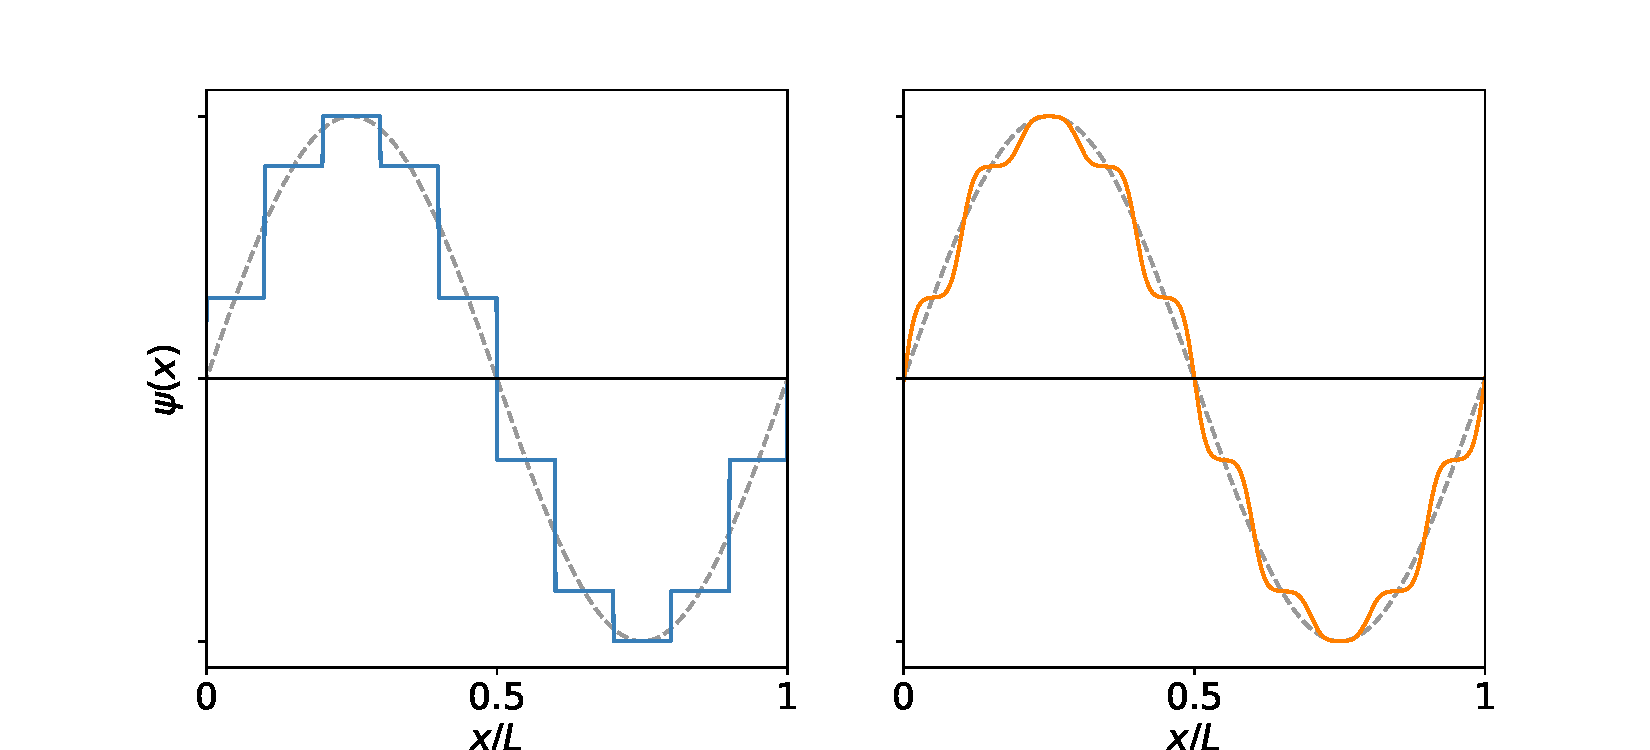
\includegraphics[width=0.9\linewidth]{\dir/img/post_smoothing}
    \caption{The effect of post-smoothing. The prolongation of the solution vector after a coarse-grid solve might look similar to the blue line in the right panel. Post-smoothing has the effect of filing off the edges of the staircase-shaped prolonged solution as depicted by the yellow line in the left panel. The prolonged error correction is then closer to the actual solution on the finer level (dashed gray line in both panels) and thus of higher quality.}
    \label{fig:post:smoothing}
\end{figure}

\subsection{Summary}

\tldr{intuitive argument}
Multigrid preconditioning of the Dirac equation as $L D \psi = L \eta$ can be seen through the following intuitive argument.
The Dirac operator is a nearest neighbor stencil.
In every iteration it is applied to the current solution vector.
Information in the current solution vector on a certain lattice site slowly propagates through the lattice; one site per iteration in each direction.
Even though the coarse Dirac operator is still nearest neighbor, information on the coarse grid travels faster through the lattice, because sites are further apart (\ie one coarse grid hop corresponds to multiple fine-grid hops depending on the choice of block size).
This enhances non-local information exchange on the lattice with fewer iterations on the coarse grid.
Additionally the coarse grid is constructed from approximate low modes which are associated to long-range interactions allowing long-distance propagation of information.
This concept is illustrated in \cref{fig:coarse:stencil}.

\begin{figure}
\centering
\includestandalone[width=0.9\linewidth]{\dir/img/long_distance}
\caption{Illustration that the coarse grid Dirac stencil transports information further through the lattice. Upper left: Dirac stencil on a $6 \times 6$ lattice connecting nearest neighbors. Instead we could restrict the vector to the coarse $3 \times 3$ grid, apply the coarse Dirac stencil (bottom center) and prolong back. The result is a longer range interaction (upper right). The information transfer is restricted to the coarse degrees of freedom, \ie the low modes of the fine grid which in turn are associated to long-range interactions. Therefore, not \emph{all} information has propagated the longer distance but the most relevant information has.}
\label{fig:coarse:stencil}
\end{figure}

\section{Multigrid propagator}
\label{sec:mg:prop}

\tldr{2-lvl MG prop decomposition}
With the definition of a coarse lattice, we can define a propagator decomposition as
\begin{equation} \label{eq:mg:prop:decomp:2lvl}
\prop = D^{-1}
= \underbrace{
  D^{-1}
  - \prolongator \coarse{D}^{-1} \restrictor
}_{\prop_0}
+ \underbrace{
  \prolongator \coarse{D}^{-1} \restrictor
}_{\prop_1}
\end{equation}
by adding and subtracting the piece along the coarse subspace.
We will generalize this equation in a recursive way by applying it repeatedly to $\coarse{D}^{-1}$ introducing $\Nlvl$ levels of multigrid.

\subsection{Recursive notation}

\tldr{all can be formulated recursively}
Before we continue, we will formulate multigrid recursively and shift in notation by defining the $\lvl$-th recursive coarse Dirac operator as coarsening of the $(\lvl-1)$-th coarse Dirac operator\footnote{The notation with the hat is clean and concise but as in real life, wearing multiple hats is awkward -- $\hat{\hat{\hat{D}}}$.}
\begin{equation}
\onlvl{D}{\lvl} = \onlvl{\restrictor}{\lvl-1} \onlvl{D}{\lvl-1} \onlvl{\prolongator}{\lvl-1} \;,
\qquad
\lvl \in \{ 1, \ldots, \Nlvl-1 \}
\end{equation}
where we define level \num{0} (also denoted as \Ln{0}) to be the fine grid
\begin{equation}
\onlvl{D}{0} = D \;,
\qquad
\onlvl{\restrictor}{0} = \restrictor \;,
\qquad
\onlvl{\prolongator}{0} = \prolongator \;.
\end{equation}
For clarity, for $\lvl = 1$, the notation changes to $\onlvl{D}{1} \equiv \coarse{D}$.
The inter-grid operators move data from and to vector spaces defined on levels $\lvl$ and $\lvl+1$
\begin{align}
\onlvl{\restrictor}{\lvl} &\colon \onlvl{\vslattice}{\lvl} \longrightarrow \onlvl{\vslattice}{\lvl+1} \;,\\
\onlvl{\prolongator}{\lvl} &\colon \onlvl{\vslattice}{\lvl+1} \longrightarrow \onlvl{\vslattice}{\lvl} \;.
\end{align}
We therefore have analogous to \cref{eq:mg:prop:decomp:2lvl} the full propagator on level $\lvl = 0, \ldots, \Nlvl-2$,
\begin{equation} \label{eq:mg:rec:prop:decomp:onlvl}
\left( \onlvl{D}{\lvl} \right)^{-1}
= \left\{ \left( \onlvl{D}{\lvl} \right)^{-1}
- \onlvl{\prolongator}{\lvl} \left( \onlvl{D}{\lvl+1} \right)^{-1} \onlvl{\restrictor}{\lvl} \right\}
+ \onlvl{\prolongator}{\lvl} \left( \onlvl{D}{\lvl+1} \right)^{-1} \onlvl{\restrictor}{\lvl} \;,
\end{equation}
with $\lvl=0$ being exactly equal to \cref{eq:mg:prop:decomp:2lvl}.
For convenience we define the compound inter-grid operators moving data directly between levels $0$ and $\lvl > 0$ as
\begin{align}
\onlvl{\mathcal{\restrictor}}{\lvl}
= \onlvl{\restrictor}{\lvl-1} \cdots \onlvl{\restrictor}{0}
\; \colon \; 
\onlvl{\vslattice}{0} \longrightarrow \onlvl{\vslattice}{\lvl} \;, \\
\onlvl{\mathcal{\prolongator}}{\lvl}
= \onlvl{\prolongator}{0} \cdots \onlvl{\prolongator}{\lvl-1}
\; \colon \; 
\onlvl{\vslattice}{\lvl} \longrightarrow \onlvl{\vslattice}{0} \;,
\end{align}
with base cases $\onlvl{\mathcal{\restrictor}}{0} = \onlvl{\mathcal{\prolongator}}{0} = \id$ for $\lvl=0$.
The recursive notation is depicted in \cref{fig:recursive:nesting}.
\begin{figure}
\centering
%\includestandalone[height=0.9\linewidth,angle=-90,origin=c]{\dir/img/nesting}
\includestandalone[width=0.9\linewidth]{\dir/img/nesting}
\caption{2D illustration of a recursive lattice coarsening. The finest lattice on level \num{0} in orange has a size of $\onlvl{V}{0}=64$. The block size for level \num{1} in green is $b_0\times b_1=2\times2$ resulting in a coarse lattice size of $\onlvl{V}{1}=16$. The coarsest lattice in purple has a trivial lattice size of $\onlvl{V}{3}=1$ and thus corresponds to LMA, where no blocking is done. The inter-grid operators $\onlvl{\restrictor}{\lvl}$ and $\onlvl{\prolongator}{\lvl}$ move data on adjacent levels, whereas the compound inter-grid operators $\onlvl{\mathcal{\restrictor}}{\lvl}$ and $\onlvl{\mathcal{\prolongator}}{\lvl}$ move data between levels \num{0} and $\lvl$. \takenfull }
\label{fig:recursive:nesting}
\end{figure}

\tldr{smoothing in recursive notation more powerful}
In this notation, pre- and post-smoother can be added to every level separately by extending the restrictors and prolongators,
\begin{align}
\onlvl{\restrictor}{\lvl} &\longrightarrow \onlvl{\restrictor}{\lvl} \onlvl{F}{\lvl}_{\text{pre}} \;, \\
\onlvl{\prolongator}{\lvl} &\longrightarrow \onlvl{F}{\lvl}_{\text{post}} \onlvl{\prolongator}{\lvl} \;,
\end{align}
with smoother acting on level $\lvl$,
\begin{align}
\onlvl{F}{\lvl}_{\text{post}} &\colon \onlvl{\vslattice}{\lvl} \longrightarrow \onlvl{\vslattice}{\lvl} \;, \\
\onlvl{F}{\lvl}_{\text{pre}} &\colon \onlvl{\vslattice}{\lvl} \longrightarrow \onlvl{\vslattice}{\lvl} \;.
\end{align}

\subsection{Propagator decomposition}

\tldr{N-lvl MG prop decomposition}
Now, we are ready to discuss a propagator decomposition using $\Nlvl$ levels of multigrid.
A general decomposition into $\Nlvl$ levels as in \cref{eq:mg:prop:decomp:2lvl} can be obtained by repeatedly plugging \cref{eq:mg:rec:prop:decomp:onlvl} into the full propagator $\prop=D^{-1}$.
With the notation from the previous section, we obtain a decomposition as
\begin{equation} \label{eq:mg:rec:prop:decomp:main}
\prop = \sum_{\lvl=0}^{\Nlvl-1} \prop_{\lvl} \;,
\end{equation}
into differences on the inner levels $\lvl < \Nlvl-1$,
\begin{equation} \label{eq:mg:rec:prop:decomp:inner:lvl}
\prop_{\lvl}
= \onlvl{\mathcal{\prolongator}}{\lvl  } \left( \onlvl{D}{\lvl  } \right)^{-1} \onlvl{\mathcal{\restrictor}}{\lvl  }
- \onlvl{\mathcal{\prolongator}}{\lvl+1} \left( \onlvl{D}{\lvl+1} \right)^{-1} \onlvl{\mathcal{\restrictor}}{\lvl+1} \;,
\end{equation}
and a single contribution on the coarsest level
\begin{equation} \label{eq:mg:rec:prop:decomp:last:lvl}
\prop_{\Nlvl-1}
= \onlvl{\mathcal{\prolongator}}{\Nlvl-1} \left( \onlvl{D}{\Nlvl-1} \right)^{-1} \onlvl{\mathcal{\restrictor}}{\Nlvl-1} \;.
\end{equation}
The equations above describe a telescoping sum, but we may consider every difference separately.

\subsection{A note on recursion}

\tldr{loop formulation more flexible}
As formalized, every subspace defined via its lattice $\onlvl{\lattice}{\lvl}$ is a valid coarsening of all its previous levels, including the fine-grid lattice $\onlvl{\lattice}{0} = \lattice$ by defining a certain block size relative to the next finer level.
A relaxed formulation of the decomposition above may allow coarse lattices to be only valid coarsenings of the fine-grid lattice.
This gives slightly higher flexibility in the choice of coarse lattices.

\tldr{example of recursive vs. loop}
As an example consider a fine-grid lattice with extents that are not powers of two, for instance $L_{\mu} = 48$.
The first level of multigrid might be chosen by a block of size $\onlvl{b}{1}_{\mu} = 4$ resulting in a coarse lattice of extents $\onlvl{L}{1}_{\mu} = 48 / 4 = 12$.
At this point, with the recursive formulation, we do not have much freedom to choose the next levels.
In \cref{tab:mg:formulations:example}, we collected possible levels in such a scenario for the recursive and the relaxed formulation.
We see the relaxed formulation allows coarse levels that are not valid coarsenings of each other, for instance \Ln{2} and \Ln{3} in \cref{tab:mg:formulations:example}, but all are valid coarsenings of the fine grid.

% The second level may be defined relative to the first level with $\onlvl{b}{2}_{\mu} = 2$ resulting in a coarse lattice of extents $\onlvl{L}{2}_{\mu} = 12 / 2 = 6$.
% This is recursive coarsening as described above.
% Clearly the second level can also be obtained by coarsening directly level \num{0} instead of level \num{1}, by defining a block of size $b_{\mu} = 8$ with respect to level \num{0}, instead of level \num{1}.
% These are two strategies to obtain the same.
% We either coarsen recursively or always relative to level \num{0}.
% The former strategy results in lattices which are always nestings of each other as depicted in \cref{fig:recursive:nesting}.
% The latter one allows more freedom in defining levels which might not always be valid coarsenings of each other.
% To catch up on the example above, instead of defining the second level as described, we could define it with a block size of $\onlvl{b}{2}_{\mu} = 6$, not with respect to the previous level but with respect to level \num{0}.
% This would result in a coarse lattice of size $\onlvl{L}{2}_{\mu} = 48 / 6 = 8$ which is still coarser than level \num{1} with $\onlvl{L}{1}_{\mu} = 12$ but cannot be obtained as direct coarsening of level \num{1}, because \num{12} is not a multiple of \num{8}.

\begin{table}
\begin{tabular}{l|ll|ll}
%\toprule
        & \multicolumn{2}{c|}{Recursive notation}           & \multicolumn{2}{c}{Relaxed notation}              \\
{Level} & {Volume}                & {Block size}            & {Volume}                & {Block size}            \\
\midrule
\Ln{0}  & $V = 48^{4}$            & -                       & $V = 48^{4}$            & -                       \\
\Ln{1}  & $\onlvl{V}{1} = 12^{4}$ & $\onlvl{b}{1} = 4^{4}$  & $\onlvl{V}{1} = 12^{4}$ & $\onlvl{b}{1} = 4^{4}$  \\
\Ln{2}  & $\onlvl{V}{2} = 6^{4}$  & $\onlvl{b}{2} = 8^{4}$  & $\onlvl{V}{2} = 8^{4}$  & $\onlvl{b}{2} = 6^{4}$  \\
\Ln{3}  & $\onlvl{V}{3} = 1^{4}$  & $\onlvl{b}{3} = 48^{4}$ & $\onlvl{V}{3} = 6^{4}$  & $\onlvl{b}{3} = 8^{4}$  \\
\Ln{4}  & -                       & -                       & $\onlvl{V}{4} = 4^{4}$  & $\onlvl{b}{4} = 12^{4}$ \\
\Ln{1}  & -                       & -                       & $\onlvl{V}{5} = 1^{4}$  & $\onlvl{b}{5} = 48^{4}$ \\
\bottomrule
\end{tabular}
\caption{
\label{tab:mg:formulations:example}
%\worktodo{caption}
Example of the recursive and relaxed formulation of multigrid.
The block size is denoted with respect to the fine grid.
The relaxed formulation allows more choice in coarse spacetime volumes.
}
\end{table}

\tldr{weird for solvers, but good for MG LMA}
The relaxed formulation might not be meaningful in a solver preconditioning scenario, where inter-grid data movement among subsequent levels is crucial for overall performance.
In terms of a propagator decomposition it indeed makes sense, not only because it provides more flexibility to fine-tune the evaluation of an observable as seen later, but also because we usually move data from and to level \num{0} and other levels.
The two variants also differ when it comes to smoothing.
The recursive variant allows control of pre- and post-smoother between all levels separately, whereas the relaxed variant only allows pre- and post-smoothing on level \num{0}.

\tldr{we use loop variant in implementation}
Implementation effort as well as performance of the two variants clearly differ and we will not discuss them further.
The implementation used for this project is the relaxed variant allowing more freedom in the coarse grid creation, \ie the one where level \num{0} is coarsened for all levels.
The formulation of the method and its subsequent analysis that will follow are independent of the choice of formulation made at this point.

% \subsection{Final propagator decomposition}

% In the decomposition of the propagator, we will allow the usage of a post-smoother not further specified.
% Therefore the final propagator on level $\lvl$ yields
% \begin{equation}
% \onlvl{\prolongator}{\lvl}_{\text{post}}
% \longrightarrow
% \onlvl{F}{\lvl}
% \onlvl{\prolongator}{\lvl}
% \end{equation}

\section{Multigrid low-mode averaging}
\label{sec:mg:lma}

We are now equipped to formulate a novel variance reduction method to evaluate $n$-point functions.

\worktodo{We note that the method will only lead to a fair variance reduction on observables sensitive to low mode noise.
The method is expected to be beneficial whenever low-mode averaging is beneficial.}

\tldr{n-pt function decomposition, grouping and illustration}
We will use the decomposition of the quark propagator established in the last section, resulting in a hierarchical $\Nlvl$-level scheme which naturally arises from the hierarchical decomposition of the fine-grid lattice.
For generality we will start with a connected $n$-point function
\begin{equation} \label{eq:Cxyz}
C(x_1;x_2;\ldots;x_n) = \tr \left\{
\propxy{x_1}{x_2}
\Gamma_1
\propxy{x_2}{x_3}
\Gamma_2
\cdots
\propxy{x_n}{x_1}
\Gamma_n
\right\} \;,
\end{equation}
where the $\Gamma_i$ are monomials of $\gamma$-matrices and the $S$ are propagators from lattice points $x_i$ to $x_j$.
Plugging in the multigrid propagator decomposition \cref{eq:mg:rec:prop:decomp:main}, we find $(\Nlvl)^{n}$ contributions
\begin{equation} \label{eq:Cijk}
C_{\lvl_1, \lvl_2, \ldots, \lvl_n}(x_1;x_2;\ldots;x_n)
= \tr \left\{
\opxy{\prop_{\lvl_1}}{x_1}{x_2}
\Gamma_1
\opxy{\prop_{\lvl_2}}{x_2}{x_3}
\Gamma_2
\cdots
\opxy{\prop_{\lvl_n}}{x_n}{x_1}
\Gamma_n
\right\} \;,
\end{equation}
indexed by the multigrid levels $\lvl_i \in \{0, \ldots, \Nlvl-1\}$, and $i \in \{1, \ldots, n\}$.
Clearly we recover the original $n$-point function \cref{eq:Cxyz} by simply summing all levels
\begin{equation}
C(x_1;x_2;\ldots;x_n)
%= \sum_{\lvl_1, \ldots, \lvl_n=0}^{\Nlvl-1}
= \sum_{\lvl_1=0}^{\Nlvl-1} \cdots \sum_{\lvl_n=0}^{\Nlvl-1}
C_{\lvl_1, \lvl_2, \ldots, \lvl_n}(x_1;x_2;\ldots;x_n) \;.
\end{equation}
Furthermore, we may define the level-$k$-contribution (also denoted as \Ln{k}) to the full correlator by collecting all components of the correlator tensor \cref{eq:Cijk}, including propagators on level $k$ or coarser but not finer levels, \ie
\begin{align}
C_{\Ln{k}}(x_1;x_2;\ldots;x_n)
= \sum_{i=1}^{n}
  \sum_{\lvl_1=k}^{\Nlvl-1}
  \ldots
  \sum_{\lvl_i=k}^{k}
  \ldots
  \sum_{\lvl_n=k+1}^{\Nlvl-1}
  % \sum_{\lvl_1, \ldots, \lvl_{i-1}, \lvl_{i+1}, \ldots, \lvl_n=k}^{\Nlvl-1}
  C_{\lvl_1, \ldots, \lvl_n}(x_1;x_2;\ldots;x_n) \;,
\end{align}
for $k \in \{0, \ldots, \Nlvl-1\}$.
The sum in $\lvl_i$ is trivial only participating one summand with $\lvl_i=k$.
Using this grouping of levels, the full correlator \cref{eq:Cxyz} can be recovered by summing over all levels,
\begin{align}
C(x_1;x_2;\ldots;x_n) = \sum_{k=0}^{\Nlvl-1} C_{\Ln{k}}(x_1;x_2;\ldots;x_n) \;.
\end{align}
This decomposition into level-contributions comes natural as illustrated in \cref{fig:mg:corr} for correlator tensors with ranks $n=1,2,3$.
% \begin{figure}
% \centering
% \includestandalone[width=0.4\linewidth]{\dir/img/mg_corr_2d}
% \caption{Grouping into contribution on multigrid levels of a $2$-point connected correlator. Elements of the correlator tensor $C_{ij}$, \cref{eq:Cijk} are assigned to grid levels \Ln{k}. The sum of the orange shaded elements correspond to the \Ln{0}-contribution of the correlator, green to \Ln{1}, red to \Ln{2} etc. Summing all tensor elements is equal to summing all levels and results in the full correlator.}
% \label{fig:mg:corr}
% \end{figure}
\begin{figure}
\centering
\subfloat[rank-$1$ tensor]{%
  \includestandalone[height=0.27\textheight]{\dir/img/mg_corr_1d}
}
\subfloat[rank-$2$ tensor]{%
  \includestandalone[height=0.27\textheight]{\dir/img/mg_corr_2d}
}
\subfloat[rank-$3$ tensor]{
  \includestandalone[height=0.27\textheight]{\dir/img/mg_corr_3d}
}
% \begin{subfigure}{0.057\textwidth}
% \includestandalone[width=\linewidth]{\dir/img/mg_corr_1d}
% \end{subfigure}
% \hfill
% \begin{subfigure}{0.45\textwidth}
% \includestandalone[width=\linewidth]{\dir/img/mg_corr_2d}
% \end{subfigure}
% \hfill
% \begin{subfigure}{0.45\textwidth}
% \includestandalone[width=\linewidth]{\dir/img/mg_corr_3d}
% \end{subfigure}
\caption{(a) Grouping into contributions of multigrid levels of a $1$-point correlator. (b) Grouping into contribution on multigrid levels of a $2$-point connected correlator into \num{8} multigrid levels. Elements of the correlator tensor $C_{ij}$, \cref{eq:Cijk} are assigned to grid levels \Ln{k}. The sum of the orange shaded elements correspond to the \Ln{0}-contribution of the correlator, green to \Ln{1}, red to \Ln{2} etc. Summing all tensor elements is equal to summing all levels and results in the full correlator. (c) Example of a $3$-point connected correlator tensor grouping into \num{4} multigrid levels. \takenpart }
\label{fig:mg:corr}
\end{figure}
Crucial about this decomposition is that every level can be evaluated separately with a different strategy in terms of number and type of sources.
An evaluation of $C_{\Ln{k}}$ requires only inversions of the Dirac operator $\onlvl{D}{k}$ on level $k$ and coarser levels but not on finer levels $0, \ldots, k-1$.
$C_{\Ln{0}}$ requires fine-grid solves.
The fact that the coarse Dirac operators have exactly the same sparsity structure as the fine one (see \cref{fig:coarse:op:structure}) allows to use the same solvers algorithms for inversions.

\section{Two-point connected correlator}
\label{sec:mg:2pt}

\tldr{2-pt example simplified heavily}
We will continue with the connected bare isovector vector current correlator in the time-momentum representation already touched upon in \cref{sec:2pt-corr,eq:G:corr:connected} -- our target observable.
Although the decomposition can be applied to any $n$-point function as seen above.
For a two-point function the formulas simplify heavily.
We have the full correlator
\begin{align} \label{eq:2pt:G}
G(t) &= \frac{1}{\lvert \Omega \rvert} \sum_{y \in \Omega} \sum_{\vect{x} \in \idxspace} C(y_0+t, \vect{x} ; y) \;,
\\
C(x; y) &= \tr \left\{ \propxy{x}{y} \Gamma_1 \propxy{y}{x} \Gamma_2 \right\} \;,
\end{align}
and the rank-2 correlator tensor
\begin{equation} \label{eq:Cij}
C_{ij}(x; y) = \tr \left\{ \opxy{\prop_{i}}{x}{y} \Gamma_1 \opxy{\prop_{j}}{y}{x} \Gamma_2 \right\} \;,
\qquad i,j \in \{0, \ldots, \Nlvl-1\} \;.
\end{equation}
The contribution into levels for a two-point function is depicted in \cref{fig:mg:corr} (b).
Therefore, the Euclidean time correlator \cref{eq:G:corr:connected} can be written as sum of level contributions
\begin{align}
G(t) = \sum_{k=0}^{\Nlvl-1} G_{\Ln{k}}(t) \;.
\end{align}

\subsection{Two-level multigrid LMA}

\tldr{2-lvl MG}
For only two multigrid levels, $\Nlvl=2$, we have a simple propagator decomposition \cref{eq:mg:prop:decomp:2lvl} and two level-contributions for the correlator
\begin{align}
&\begin{aligned}
C_{\Ln{0}}(x;y)
&= C(x;y) - C_{\Ln{1}}(x;y) \\
&= \tr \left\{ \opxy{\prop}{x}{y} \Gamma_1 \opxy{\prop}{y}{x} \Gamma_2 \right\}
 - \tr \left\{ \opxy{\prop_{1}}{x}{y} \Gamma_1 \opxy{\prop_{1}}{y}{x} \Gamma_2 \right\} \;,
\end{aligned} \\
&C_{\Ln{1}}(x;y)
= \tr \left\{ \opxy{\prop_{1}}{x}{y} \Gamma_1 \opxy{\prop_{1}}{y}{x} \Gamma_2 \right\} \;.
\end{align}
The Euclidean time correlator enjoys the same decomposition
\begin{equation}
G(t) = G_{\Ln{0}}(t) + G_{\Ln{1}}(t) \;,
\end{equation}
where we can choose different evaluation strategies for the two terms.
Clearly for every sample of the fine-grid \Ln{0}-term we have to solve the full Dirac equation, $D \psi = \eta$ for some source $\eta$, whereas for the coarse-grid \Ln{1}-term we have to solve the coarse Dirac equation $\coarse{D} \coarse{\psi} = \coarse{\eta}$ for some coarse source $\coarse{\eta}$ in the smaller subspace $\coarse{\vslattice}$.
Solving the coarse system is significantly cheaper than solving the fine-grid system if the subspace was chosen properly.
This is, if the coarse dimension is much smaller than the fine one, $\dim_{\mathbb{C}}(\coarse{\vslattice}) \ll \dim_{\mathbb{C}}(\vslattice)$.
Our strategy will be as follows: the expensive \Ln{0}-term will be evaluated with as few as possible sources, for instance \numrange{1}{10}, whereas the cheap \Ln{1}-term will be sampled with many sources, say \numrange{100}{1000}.
We will present different estimators for the level contributions, but every estimator that is valid on the fine-grid correlator can be safely used on coarse levels too.

\subsection{Point-source estimator on level $k$}

\worktodo{todo}

\subsection{Stochastic estimator on level $k$}

\tldr{stochastic estimator on lvl similar to plain stochastic estimator}
As introduced in \cref{sec:stochastic:prop} we may use a stochastic estimator for level $k$.
By using \cref{eq:stoch:C:full} as basis we plug in the propagator decomposition.
The final equation only changes slightly by replacing the propagator $\prop$ with the propagators on the involved levels
\begin{align}
% C_{ij}(x_0, y_0)
% &\approx \frac{1}{\Nst} \sum_{n=0}^{\Nst-1} \sum_{\vect{x}} \;
% \sprod{
%   \fieldx{(\prop_j \gamma^{5} \eta_n^{\tslice{y_0}})}{x}
% }{
%   \gamma^{5}
%   \Gamma_2
%   \fieldx{(\prop_i \Gamma_1 \eta_n^{\tslice{y_0}})}{x}
% } \;,
C_{ij,n}(x_0, y_0)
&= \frac{1}{L^{3}} \sum_{\vect{x}} \;
\sprod{
  \fieldx{(\prop_j \gamma^{5} \eta_n^{\tslice{y_0}})}{x}
}{
  \gamma^{5}
  \Gamma_2
  \fieldx{(\prop_i \Gamma_1 \eta_n^{\tslice{y_0}})}{x}
} \;,
\end{align}
compare \cref{eq:stoch:C:full}.
Evaluating the above, requires us to solve the linear systems of equation
\begin{align}
\onlvl{D}{\lvl  }
\psi_{n}^{\Gamma \tslice{t} (\lvl)} &=
\onlvl{\mathcal{\restrictor}}{\lvl  }
\Gamma \eta_n^{\tslice{t}} \;,
\end{align}
on levels $\lvl = i, j, i+1, j+1$ and time-slice $t$ analogous to \cref{eq:stoch:C:solves}.
According to \cref{eq:mg:rec:prop:decomp:inner:lvl}, the fine-grid stochastic propagator is evaluated as prolonged differences of these solves,
\begin{align} \label{eq:prolonged:solves}
\phi_{n(\lvl)}^{\Gamma \tslice{t}}
&= S_{\lvl} \Gamma \eta_n^{\tslice{t}}
% \\
% &= \onlvl{\mathcal{\prolongator}}{\lvl  }
%   \left( \onlvl{D}{\lvl  } \right)^{-1}
%   \onlvl{\mathcal{\restrictor}}{\lvl  }
%   \Gamma \eta_n^{\tslice{t}}
% - \onlvl{\mathcal{\prolongator}}{\lvl+1}
%   \left( \onlvl{D}{\lvl+1} \right)^{-1}
%   \onlvl{\mathcal{\restrictor}}{\lvl+1}
%   \Gamma \eta_n^{\tslice{t}}
% \\
= \onlvl{\mathcal{\prolongator}}{\lvl  }
  \psi_{n}^{\Gamma \tslice{t} (\lvl)}
- \onlvl{\mathcal{\prolongator}}{\lvl+1}
  \psi_{n}^{\Gamma \tslice{t} (\lvl+1)} \;, \\
\phi_{n(\Nlvl-1)}^{\Gamma \tslice{t}}
&= S_{\Nlvl-1} \Gamma \eta_n^{\tslice{t}}
= \onlvl{\mathcal{\prolongator}}{\Nlvl-1  }
  \psi_{n}^{\Gamma \tslice{t} (\Nlvl-1)} \;,
\end{align}
for $\lvl < \Nlvl-1$, where the coarsest level contribution has no subtracted term.
The final term can be written in terms of the prolonged differences \cref{eq:prolonged:solves} -- a scalar product in the fine-grid as
\begin{align}
% C(x_0, y_0)
% &\approx \frac{1}{\Nst} \sum_{n=0}^{\Nst-1} \sum_{\vect{x}} \;
% \sprod{
%   \fieldx{\psi_{n}^{\gamma^{5} \tslice{y_0}}}{x}
% }{
%   \gamma^{5}
%   \gamma_k
%   \fieldx{\psi_{n}^{\gamma_k \tslice{y_0}}}{x}
% }. \\
% C_{ij}(x_0, y_0)
% &\approx
% % \frac{1}{\Nst} \sum_{n=0}^{\Nst-1} \sum_{\vect{x}} \;
% % \sprod{
% %   \fieldx{(\prop_j \gamma^{5} \eta_n^{\tslice{y_0}})}{x}
% % }{
% %   \gamma^{5}
% %   \Gamma_2
% %   \fieldx{(\prop_i \Gamma_1 \eta_n^{\tslice{y_0}})}{x}
% % } \\
% % &=
% \frac{1}{\Nst} \sum_{n=0}^{\Nst-1} \sum_{\vect{x}} \;
% \sprod{
%   \fieldx{\phi_{n(j)}^{\gamma^{5} \tslice{y_0}}}{x}
% }{
%   \gamma^{5}
%   \Gamma_2
%   \fieldx{ \phi_{n(i)}^{\Gamma_1 \tslice{y_0}} }{x}
% } \;.
C_{ij,n}(x_0, y_0)
&=
\frac{1}{L^{3}} \sum_{\vect{x}} \;
\sprod{
  \fieldx{\phi_{n(j)}^{\gamma^{5} \tslice{y_0}}}{x}
}{
  \gamma^{5}
  \Gamma_2
  \fieldx{ \phi_{n(i)}^{\Gamma_1 \tslice{y_0}} }{x}
} \;.
\end{align}
compare \cref{eq:stoch:C:full:final} or directly in terms of the coarse spinor solutions
% \begin{align}
% C_{ij}(x_0, y_0)
% &\approx
% \frac{1}{\Nst} \sum_{n=0}^{\Nst-1} \sum_{\vect{x}} \;
% \sprod{
%   \fieldx{\phi_{n(j)}^{\gamma^{5} \tslice{y_0}}}{x}
% }{
%   \gamma^{5}
%   \Gamma_2
%   \fieldx{ \phi_{n(i)}^{\Gamma_1 \tslice{y_0}} }{x}
% } \\
% \phi_{n(i)}^{\Gamma_1 \tslice{y_0}}
% &= \onlvl{\mathcal{\prolongator}}{i}
%   \psi_{n}^{\Gamma_1 \tslice{y_0} (i)}
% - \onlvl{\mathcal{\prolongator}}{i+1}
%   \psi_{n}^{\Gamma_1 \tslice{y_0} (i+1)} \\
% \phi_{n(j)}^{\gamma^{5} \tslice{y_0}}
% &= \onlvl{\mathcal{\prolongator}}{j}
%   \psi_{n}^{\gamma^{5} \tslice{y_0} (j)}
% - \onlvl{\mathcal{\prolongator}}{j+1}
%   \psi_{n}^{\gamma^{5} \tslice{y_0} (j+1)} \\
% C_{ij}(x_0, y_0)
% &\approx
% \frac{1}{\Nst} \sum_{n=0}^{\Nst-1} \sum_{\vect{x}} \;
% \sprod{
%   \fieldx{\phi_{n(j)}^{\gamma^{5} \tslice{y_0}}}{x}
% }{
%   \gamma^{5}
%   \Gamma_2
%   \fieldx{(\onlvl{\mathcal{\prolongator}}{i} \psi_{n}^{\Gamma_1 \tslice{y_0} (i)})}{x}
% } \\
% &-
% \sprod{
%   \fieldx{\phi_{n(j)}^{\gamma^{5} \tslice{y_0}}}{x}
% }{
%   \gamma^{5}
%   \Gamma_2
%   \fieldx{(\onlvl{\mathcal{\prolongator}}{i+1} \psi_{n}^{\Gamma_1 \tslice{y_0} (i+1)})}{x}
% } \\
% &=
% \frac{1}{\Nst} \sum_{n=0}^{\Nst-1} \sum_{\vect{x}} \;
% \sprod{
%   \fieldx{(\onlvl{\mathcal{\prolongator}}{j} \psi_{n}^{\gamma^{5} \tslice{y_0} (j)})}{x}
% }{
%   \gamma^{5}
%   \Gamma_2
%   \fieldx{( \onlvl{\mathcal{\prolongator}}{i}\psi_{n}^{\Gamma_1 \tslice{y_0} (i)})}{x}
% } \\
% &-
% \sprod{
%   \fieldx{( \onlvl{\mathcal{\prolongator}}{j+1}\psi_{n}^{\gamma^{5} \tslice{y_0} (j+1)})}{x}
% }{
%   \gamma^{5}
%   \Gamma_2
%   \fieldx{( \onlvl{\mathcal{\prolongator}}{i}\psi_{n}^{\Gamma_1 \tslice{y_0} (i)})}{x}
% } \\
% &-
% \sprod{
%   \fieldx{( \onlvl{\mathcal{\prolongator}}{j}\psi_{n}^{\gamma^{5} \tslice{y_0} (j)})}{x}
% }{
%   \gamma^{5}
%   \Gamma_2
%   \fieldx{( \onlvl{\mathcal{\prolongator}}{i+1}\psi_{n}^{\Gamma_1 \tslice{y_0} (i+1)})}{x}
% } \\
% &+
% \sprod{
%   \fieldx{( \onlvl{\mathcal{\prolongator}}{j+1}\psi_{n}^{\gamma^{5} \tslice{y_0} (j+1)})}{x}
% }{
%   \gamma^{5}
%   \Gamma_2
%   \fieldx{( \onlvl{\mathcal{\prolongator}}{i+1}\psi_{n}^{\Gamma_1 \tslice{y_0} (i+1)})}{x}
% } \\
% \end{align}
\begin{multline}
% C_{ij}(x_0, y_0)
% \approx
% \frac{1}{\Nst} \sum_{n=0}^{\Nst-1} \sum_{\lvl_1 \in \mathcal{A}_i} \sum_{\lvl_2 \in \mathcal{A}_j} \;
% (-1)^{i+j + \lvl_1 + \lvl_2} \\
% \cdot \sum_{\vect{x}} \sprod{
%   \fieldx{( \onlvl{\mathcal{\prolongator}}{\lvl_2}\psi_{n}^{\gamma^{5} \tslice{y_0} (\lvl_2)})}{x}
% }{
%   \gamma^{5}
%   \Gamma_2
%   \fieldx{( \onlvl{\mathcal{\prolongator}}{\lvl_1}\psi_{n}^{\Gamma_1 \tslice{y_0} (\lvl_1)})}{x}
% } \;,
C_{ij,n}(x_0, y_0)
= \frac{1}{L^{3}}
\sum_{\lvl_1 \in \mathcal{A}_i} \sum_{\lvl_2 \in \mathcal{A}_j} \;
(-1)^{i+j + \lvl_1 + \lvl_2} \\
\cdot \sum_{\vect{x}} \sprod{
  \fieldx{( \onlvl{\mathcal{\prolongator}}{\lvl_2}\psi_{n}^{\gamma^{5} \tslice{y_0} (\lvl_2)})}{x}
}{
  \gamma^{5}
  \Gamma_2
  \fieldx{( \onlvl{\mathcal{\prolongator}}{\lvl_1}\psi_{n}^{\Gamma_1 \tslice{y_0} (\lvl_1)})}{x}
} \;,
\end{multline}
where the index set $\mathcal{A}_\lvl$ is defined as
\begin{equation}
\mathcal{A}_\lvl = \{\lvl,\lvl+1\} \cap \{0, \ldots, \Nlvl-1\} \;.
\end{equation}
The final estimator using $\Nst$ stochastic time-diluted fine-grid wall-sources $\eta_n^{\tslice{t_n}}$ with support on time-slice $t_n$ chosen uniformly from $\{0, \ldots, L_0 - 1\}$ is
\begin{align} \label{eq:stoch:Gij:final}
G_{\Ln{k}}(t) &= G_{kk}(t) + \sum_{i=k+1}^{\Nlvl-1} \Big( G_{ik}(t) + G_{ki}(t) \Big) \;, \\
G_{ij}(t) &= \frac{1}{\Nst} \sum_{n=0}^{\Nst-1} C_{ij,n}(t+t_n;t_n) \;.
\end{align}

%This is an estimator with $\Nst$ stochastic time-diluted fine-grid wall-sources $\eta_n^{\tslice{t_n}}$ with support on time-slice $t_n$ chosen uniformly from $\{0, \ldots, L_0 - 1\}$.

\tldr{spin sources only 4 inversion, no matter the spin structure}
We will use spin-diagonal random wall-sources~\cite{ETM:2008zte} allowing an unbiased estimator for each spin matrix element separately.
The full spin structure of the correlator given by $\Gamma_1$ and $\Gamma_2$ can be reconstructed using only \num{4} spin-diagonal stochastic sources.
In total, this amounts $4 \Nst$ inversions per noise-source, no matter the $\gamma$-structure.
For $\prop_i = \prop_j = \prop$, this is just the usual stochastic estimator for the two-point correlator.
It is straightforward to generalize to other source types.

\tldr{sources cascade down, but not up}
We want to emphasize that a stochastic sample of level $\lvl$ also requires solves on all coarser levels.
However this gives us a stochastic sample on all coarser levels too.
We may use the same stochastic source as sample on multiple levels, since these are independent traces.

% \begin{align}
% C_{ij}(x_0, y_0)
% &= \sum_{\vect{x}, \vect{y}} \;
% \tr \left\{ \propxy{x}{y}^i \Gamma_1 \propxy{y}{x}^j \Gamma_2 \right\} \\
% &= \sum_{\vect{x}, w, z} \;
% \tr \left\{
%   \propxy{x}{w}^i \Gamma_1
%   \opxy{\id^{\tslice{y_0}}_{\text{st}}}{w}{z}
%   \propxy{z}{x}^j \Gamma_2
% \right\} \\
% &\approx \frac{1}{\Nst} \sum_{n=0}^{\Nst-1} \sum_{\vect{x}, w, z} \;
% \tr \left\{
%   \propxy{x}{w}^i \Gamma_1
%   \fieldx{\eta_n^{\tslice{y_0}}}{w}
%   (\fieldx{\eta_n^{\tslice{y_0}}}{z})^{\dagger}
%   \propxy{z}{x}^j \Gamma_2
% \right\} \\
% &= \frac{1}{\Nst} \sum_{n=0}^{\Nst-1} \sum_{\vect{x}, w, z} \;
% \tr \left\{
%   \propxy{x}{w}^i \Gamma_1
%   \fieldx{\eta_n^{\tslice{y_0}}}{w}
%   (\opxy{\prop_j^{\dagger}}{x}{z} \fieldx{\eta_n^{\tslice{y_0}}}{z})^{\dagger}
%   \Gamma_2
% \right\} \\
% &= \frac{1}{\Nst} \sum_{n=0}^{\Nst-1} \sum_{\vect{x}} \;
% \tr \left\{
%   \fieldx{(\prop_i \Gamma_1
%   \eta_n^{\tslice{y_0}})}{x}
%   \fieldx{(\prop_j^{\dagger} \eta_n^{\tslice{y_0}}}{x})^{\dagger}
%   \Gamma_2
% \right\} \\
% &= \frac{1}{\Nst} \sum_{n=0}^{\Nst-1} \sum_{\vect{x}} \;
% \tr \left\{
%   \fieldx{(\prop_j^{\dagger} \eta_n^{\tslice{y_0}}}{x})^{\dagger}
%   \Gamma_2
%   \fieldx{(\prop_i \Gamma_1
%   \eta_n^{\tslice{y_0}})}{x}
% \right\} \\
% &= \frac{1}{\Nst} \sum_{n=0}^{\Nst-1} \sum_{\vect{x}} \;
% \sprod{
%   \fieldx{(\prop_j^{\dagger} \eta_n^{\tslice{y_0}}}{x})
% }{
%   \fieldx{(\Gamma_2 \prop_i \Gamma_1 \eta_n^{\tslice{y_0}})}{x}
% } \\
% &= \frac{1}{\Nst} \sum_{n=0}^{\Nst-1} \sum_{\vect{x}} \;
% \sprod{
%   \fieldx{(\prop_j \gamma^{5} \eta_n^{\tslice{y_0}}}{x})
% }{
%   \gamma^{5}
%   \Gamma_2
%   \fieldx{(\prop_i \Gamma_1 \eta_n^{\tslice{y_0}})}{x}
% }
% \end{align}


\subsection{Exact estimator on coarsest level}
\label{sec:mglma:coarsest:exact}

\tldr{formulas for exact coarsest lvl}
When estimating the coarsest grid contribution, its dimension might be small enough for an exact estimation.
This is the case if its dimension no larger than say $10^{4}$.
The coarsest term can then be brought into a simpler form
\begin{multline} \label{eq:mglma:coarsest:exact}
G_{\Ln{(\Nlvl-1)}}(t)
= \frac{1}{\lvert \idxspacetime \rvert} \sum_{y_0=0}^{L_0-1} \\
\cdot \tr \left\{
  (\onlvl{D}{\Nlvl-1})^{-1}
  \fieldx{\onlvl{\Gamma_1}{\Nlvl-1}}{y_0}
  (\onlvl{D}{\Nlvl-1})^{-1}
  \fieldx{\onlvl{\Gamma_2}{\Nlvl-1}}{t+y_0}
\right\} \;.
\end{multline}
The $\Gamma$-matrices are defined as in \cref{eq:coarse:index} as coarsened operators with the time extent as open index, \ie defined with a partial trace over space $\idxspace$, color $\idxcolor$ and spin $\idxspin$ but not time, see \cref{eq:partial:trace}.
Explicitly
\begin{equation} \label{eq:gamma:partial:trace}
\left( \onlvl{\Gamma_k}{\Nlvl-1} \right)_{ij} = \tr_{\idxspace \times \idxspin \times \idxcolor} \left( \Gamma_k \phi_j \phi_i^\dagger \right) \;.
\end{equation}

\tldr{compare to full-vol averaged corr}
The trace in \cref{eq:mglma:coarsest:exact} is over all coarse degrees of freedom present on the coarse grid.
The fine-grid spacetime dependency in the trace is shifted into the coarse $\Gamma$-matrices making a full lattice volume average straightforward.
Let us compare this form with the full lattice volume averaged correlator $\lvert \Omega \lvert = \lvert \idxspacetime \lvert$ on the fine grid,
\begin{equation} \label{eq:G:corr:volume:averaged}
\mathcal{G}(t) =
\frac{1}{\lvert \idxspacetime \rvert}
\sum_{y \in \idxspacetime}
\sum_{\vect{x}} \;
\tr \left\{
  \propxy{t+y_0, \vect{x}}{y} \Gamma_1 \propxy{y}{t+y_0, \vect{x}} \Gamma_2
\right\} \;.
\end{equation}
We see that it has exactly the same form, just with some replacements.
The fine-grid $\Gamma$-matrices are replaced with the coarse ones, the fine-grid inverse Dirac operator $\prop=D^{-1}$ is replaced with the coarse one $(\onlvl{D}{\Nlvl-1})^{-1}$ and finally the trace over color, spin and space is replaced by a trace over coarse color, spin and space.
Note that the original fine-grid trace over color, spin and space is moved to the $\Gamma$-matrices \cref{eq:gamma:partial:trace}.
However, the term is calculated exactly and averaged over the full spacetime volume, its variance will be minimal, \ie the gauge variance of that level.

\tldr{LMA does exact coarsest lvl, but without blocking}
Revisiting low-mode averaging one more time, we notice that the above form is exactly equal to the eigen-eigen term of low-mode averaging worked out in \cref{eq:Gconn:eigen-eigen}, if the coarsest lattice is trivial.
To see this, we remember the conclusions drawn in \cref{sec:sd:lma} and write the trace in index notation. 
Then \cref{eq:mglma:coarsest:exact} turns quickly into
\begin{equation}
% G_{\Ln{1}}(t)
% = \frac{1}{\lvert \idxspacetime \rvert} \sum_{y_0=0}^{L_0-1}
% \tr \left\{
%   \coarse{Q}^{-1}
%   \coarse{\gamma^{5} \Gamma_1}(y_0)
%   \coarse{Q}^{-1}
%   \coarse{\gamma^{5} \Gamma_2}(t+y_0)
% \right\} \;.
G_{\Ln{1}}(t)
= \frac{1}{\lvert \idxspacetime \rvert} \sum_{y_0=0}^{L_0-1}
\sum_{k,l,m,n}
(\coarse{Q}^{-1})_{[kl]}
\left( \fieldx{\coarse{\gamma^{5} \Gamma_1}}{y_0} \right)_{[lm]}
(\coarse{Q}^{-1})_{[mn]}
\left( \fieldx{\coarse{\gamma^{5} \Gamma_2}}{t+y_0} \right)_{[nk]} \;.
\end{equation}
Using the fact that in case of low-mode averaging the coarse Hermitian Dirac operator $\coarse{Q}$ is diagonal with eigenvalues along its diagonal, $(\coarse{Q}^{-1})_{[kl]} = \delta_{kl} \lambda_k^{-1}$, and reversing the definition of the coarse $\Gamma$-matrices as in \cref{eq:coarse:index};
\begin{multline}
G_{\Ln{1}}(t)
= \frac{1}{\lvert \idxspacetime \rvert} \sum_{y_0=0}^{L_0-1} \sum_{k,m}
\frac{1}{\lambda_k \lambda_m}
\sum_{\vect{y}}
%\left( \fieldx{\coarse{\gamma^{5} \Gamma_1}}{y_0} \right)_{[lm]}
\sprod{
  \fieldx{\phi_l}{y}
}{
  \gamma^{5}
  \Gamma_1
  \fieldx{\phi_m}{y}
} \\
\cdot \sum_{\vect{x}}
%\left( \fieldx{\coarse{\gamma^{5} \Gamma_2}}{t+y_0} \right)_{[nk]}
\sprod{
  \fieldx{\phi_n}{t+y_0,\vect{x}}
}{
  \gamma^{5}
  \Gamma_2
  \fieldx{\phi_k}{t+y_0,\vect{x}}
} \,,
\end{multline}
we readily find \cref{eq:Gconn:eigen-eigen} identically, with the bootstrap vectors chosen as low modes $\phi_i = \evec_i$ as is done in LMA.

\tldr{terminating lvl is LMA}
In fact even in a multigrid scenario with more than \num{2} levels, one has the freedom to choose the coarsest lattice to be trivial resulting in a final layer of traditional low-mode averaging.
Even though such a layer does add only negligible cost, it is only useful for small enough lattices as we will see in the numerical study in \cref{ch:p2:numerics}.

\subsection{$V^2$ problem of LMA}

\worktodo{where to put this?}

\subsection{Cross-term problem of LMA}

\worktodo{where to put this?}

\worktodo{Motivated by the previous sections and the results in refs. \cite{Clark_2018, Alcalde_2017}, we want to use the subspace $\coarse{\vslattice}$ generated from the lattice $\coarse{\lattice} = (\coarse{\idxspacetime}, \coarse{\idxspin}, \coarse{\idxcolor})$ as averaging- or sample-subspace in our LMA-scenario.}

\section{Summary}
\label{sec:mg:summary}

\tldr{summary MG as preconditioner}
As a preliminary foundation, we looked at multigrid as a preconditioner which is specially powerful on ill-conditioned systems, because of the low-mode suppression inherent to Krylov solvers.
Multigrid scales close to linear in the lattice volume, even though the dimension of the low-mode subspace does so too.
Low-mode error components in the iterative solution are treated by solving the coarse Dirac equation to low precision in every outer Krylov iteration.

\tldr{summary MG as prop decomposition}
The quark propagator (the inverse of the Dirac operator) can be decomposed into a contribution along the multigrid subspace and a remainder.
This can be repeated recursively, leading to a decomposition of an arbitrary $n$-point function into $\Nlvl$ multigrid level contributions in a natural way.
Every level can be evaluated individually with a different evaluation strategy.
Low-mode averaging is a special case of this decomposition with a trivial coarse lattice.

% \worktodo{
%   * Krylov solvers supress low mode contributions
%   * V2 problem
%   * MG solves the coarse Dirac equation to low precision in every outer iteration
%   * with this a MG propagator decomposition can be written down
%   * recusively
%   * Every n-point function can be decomposed into levels in a natural way
%   * Every level evaluated with a different strategy
%   * 
% }
